\chapter{Utilisation du solveur Choco}
\label{annexe:choco}

Cette annexe présente les éléments utiles pour réaliser le TP sur les mobiles
avec le solveur Choco, écrit en Java. Pour plus de renseignements, se référer
au site:\\
\centerline{\url{http://www.emn.fr/z-info/choco-solver/index.html}}

%%NB : Afin de simplifier la prise en main rapide du solveur, certaines signatures de méthodes ont été modifiées par rapport à la documentation du solveur pour n'accepter que certains sous-types intéressants pour le TP.

\subsection*{Faire appel à la bibliothèque Choco}

La bibliothèque Choco est disponible sous forme de .jar. Sous l'environnement
de développement pour Java ECLiPSe, il suffit d'inclure le chemin vers la
bibliothèque dans le classpath du projet (menu Project, Properties, Java Build
Path, onglet Libraries, bouton Add External JARs \ldots).\\
Il faut importer en tête de fichier les classes de Choco qui seront utilisées.
Dans notre cas:\\
\texttt{import static choco.Choco.*;}
%%\texttt{import choco.integer.IntDomainVar;}

\subsection*{Architecture générale choco}
On identifie clairement deux parties différentes sur le schéma \ref{choco}:
\begin{enumerate}
\item modélisation du problème via la classe Model
%%\begin{itemize}
%%\item variables
%%\item contraintes
%%\end{itemize}
\item résolution du problème via la classe Solver
\end{enumerate}

\begin{figure}[!ht]
\begin{center}
%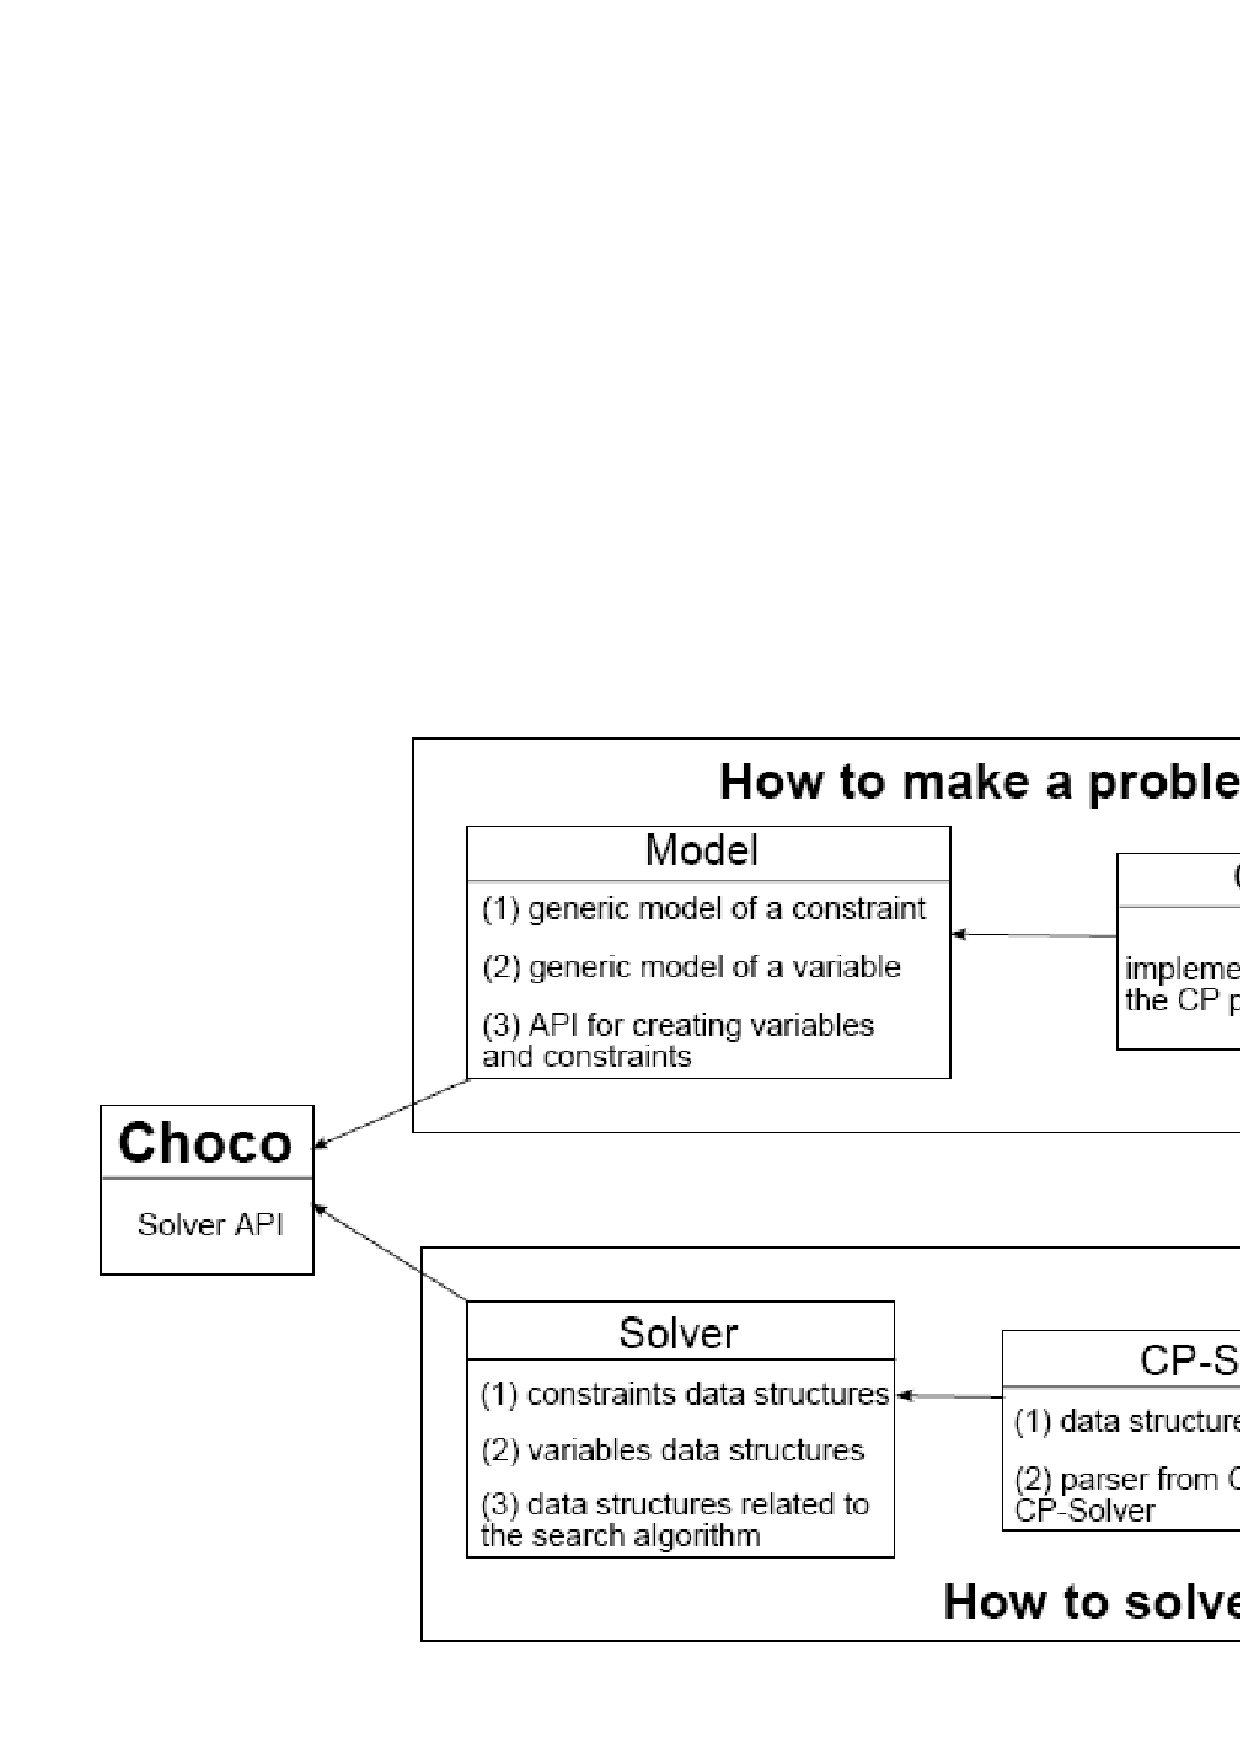
\includegraphics[width=16cm,height=6cm]{choco.pdf}
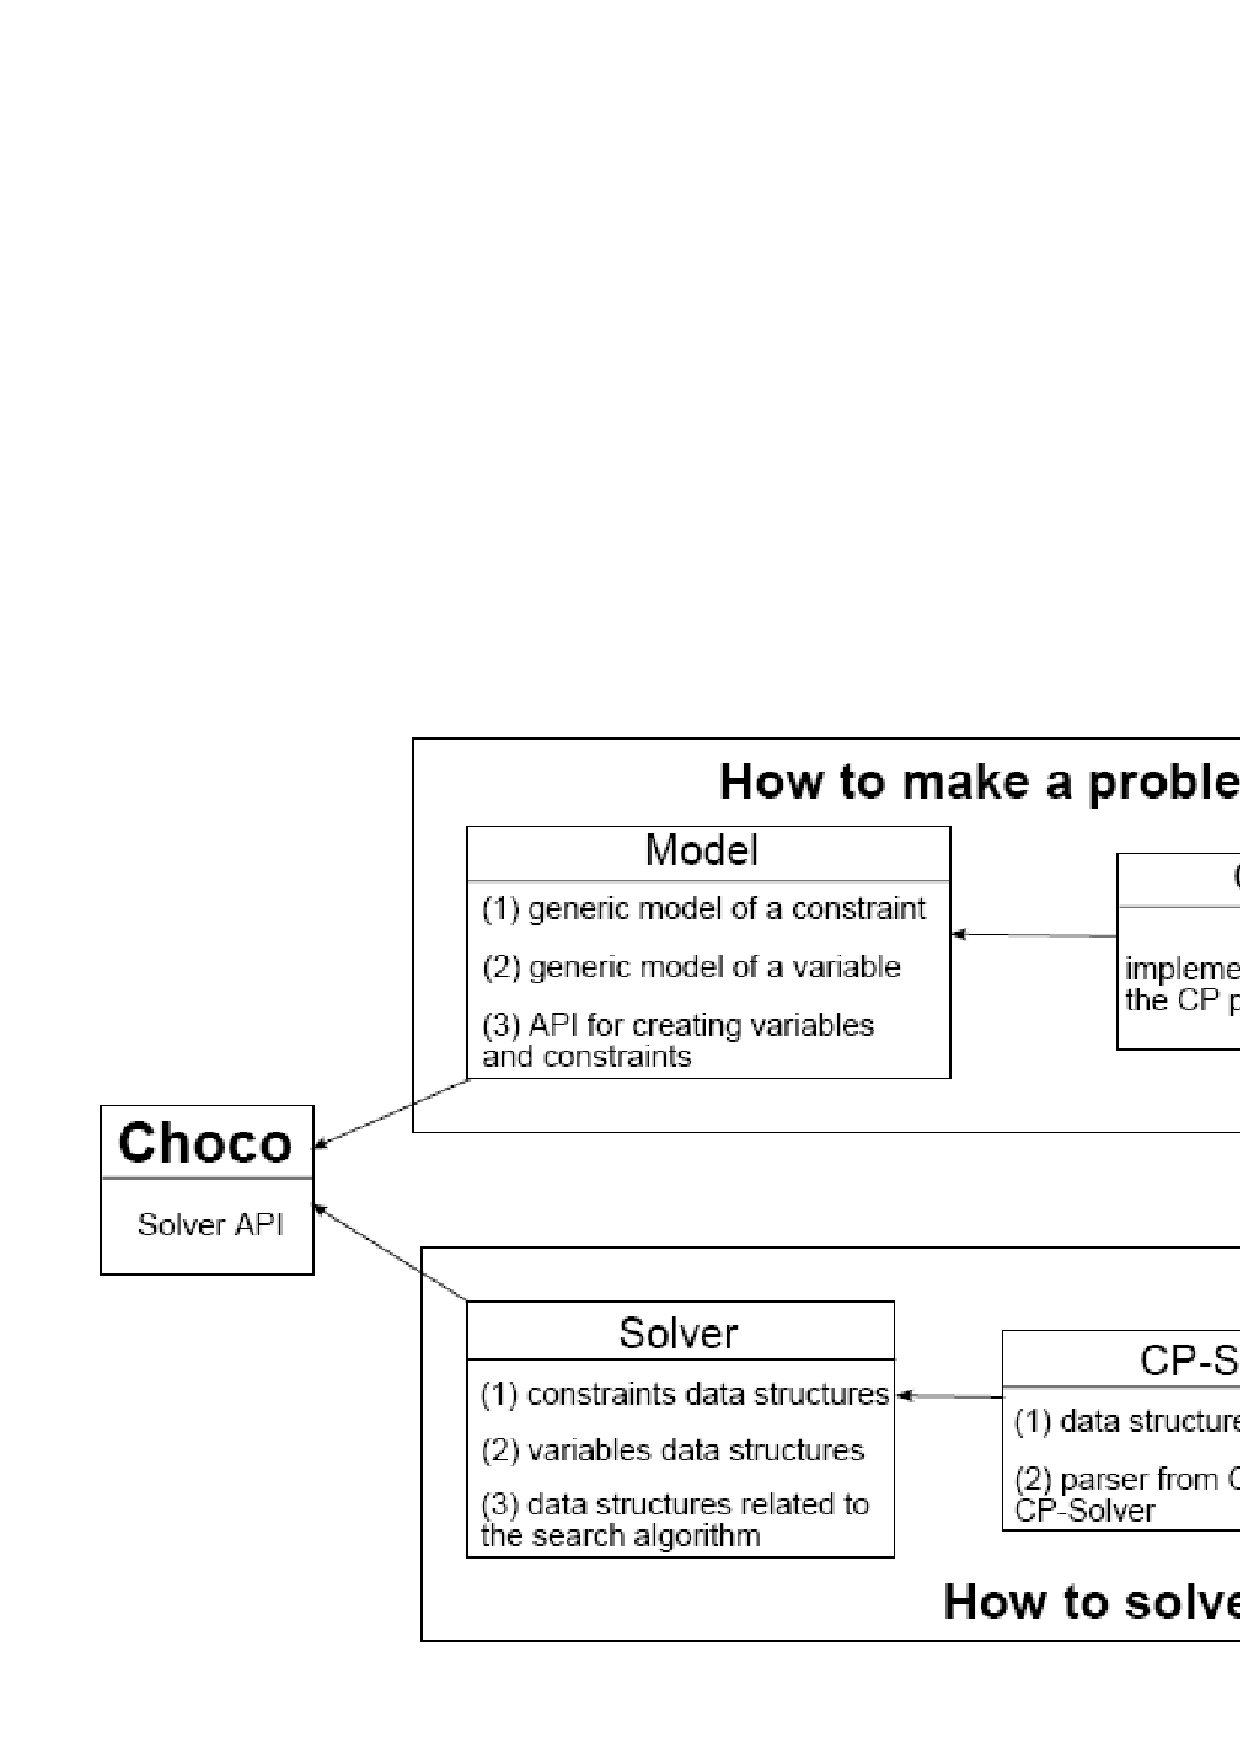
\includegraphics[width=\linewidth]{choco.pdf}
\caption{Architecture choco}
\label{choco}
\end{center}
\end{figure}
Détaillons ces étapes.


\subsection*{Modéliser un problème}
En Choco, le problème à résoudre par programmation par contraintes est une instance de la classe \texttt{Model}.\\
Constructeur d'un objet de type \texttt{Model} : \texttt{CPModel()}

\`A un objet de type \texttt{Model}, on associe:
\begin{enumerate}

\item des variables. Dans notre cas, il s'agit de variables entières à domaine
      fini.

  \begin{itemize}

  \item Déclaration:\\
  \hspace{0.5 cm} \texttt{IntegerVariable makeIntVar(String nom,int borne\_min,int borne\_max)}\\
     où \texttt{nom} est le nom de la variable, \texttt{borne\_min} et
     \texttt{borne\_max} sont les bornes inférieure et supérieure de son domaine
     de définition.

  \item Association à l'objet \texttt{Model}:\\
  \hspace{0.5 cm} \texttt{void Model$\colon\colon$addVariable(IntegerVariable var);}
  \end{itemize}

  \item des contraintes.

  \begin{itemize}
  \item Déclaration: on dispose d'un large panel de contraintes. Les plus
        utiles sont listées dans le paragraphe ci-dessous.

  \item Association à un objet \texttt{Model}:

  \hspace{0.5 cm} \texttt{void Model$\colon\colon$addConstraint(Constraint c);}
  \end{itemize}

\end{enumerate}

Imports en tête de fichier : \texttt{import choco.cp.model.CPModel;}\\
\texttt{import choco.kernel.model.variables.integer.IntegerVariable;}

\subsection*{Exprimer une contrainte}

Les contraintes sont exprimées sur des instances de la classe
\texttt{IntegerExpressionVariable}. Cette classe permet de représenter des
expressions linéaires entières (nous le notons par la suite IEV pour des
raisons de lisibilité). La classe représentant les variables sur les domaines
finis est \texttt{IntegerVariable}, elle hérite de
\texttt{IntegerExpressionVariable}.

\noindent Opération d'addition et de multiplication :\\
\texttt{IEV plus(IEV t1, IEV t2)}\\
\texttt{IEV mult(int i, IEV t)}

\noindent Contrainte d'égalité :\\
\texttt{Constraint eq(IEV t1, IEV t2)}

\noindent Contrainte de stricte infériorité :\\
\texttt{Constraint lt(IEV t1, IEV t2)}

\noindent Contrainte allDifferent :\\
\texttt{Constraint allDifferent(IV[] tab)}\\
\indent où \texttt{tab} contient les variables dont on veut contraindre les
        valeurs à être toutes différentes

\subsection*{Résoudre un problème}

Afin de résoudre un problème, on va déclarer un solveur, instance de la classe
\texttt{Solver}, et l'associer au modèle.

Constructeur d'un objet de type \texttt{Solver} :\\
\texttt{CPSolver()}

Lecture du modèle par le solveur:\\
\texttt{void Solver$\colon\colon$read(Model model)}

Lancer la résolution du système de contraintes :\\
\texttt{java.lang.Boolean Solver$\colon\colon$solve()}\\
\indent rend vrai si une solution est trouvée. Les variables sous contraintes
        sont instanciées avec les valeurs formant cette solution.

Trouver une nouvelle solution :\\
\texttt{java.lang.Boolean Solver$\colon\colon$nextSolution()}\\
\indent rend vrai si une nouvelle solution est trouvée.

Il n'est pas possible d'accéder à la valeur ou au domaine d'une variable
lorsque le processus de résolution a été appliqué par l'intermédiaire du
modèle (l'instance \texttt{Model}). Il faut pour cela utiliser le solveur.

Récupérer le domaine de la variable :\\
\texttt{IntDomainVar Solver$\colon\colon$getVar(IEV var)}

Accéder à la valeur si instanciée (valeur pour la solution courante):\\
\texttt{int IntDomainVar$\colon\colon$getVal()}

Import en tête de fichier :\\
\texttt{import choco.cp.solver.CPSolver;}
